\section{实战操作指南}
\label{sec:appendix-cloud-deploy}

本附录汇集了第五章涉及的动手操作内容，包括云端部署流程、Dockerfile逐行解读以及Kubernetes部署实战，供读者在理解原理之后按需查阅。

\subsection{云端部署操作指南}

本节提供将游戏服务器部署到云端的具体操作步骤。在阅读本节之前，建议先理解第五章中关于物理机与云主机、虚拟化原理以及云计算抽象层次的概念。

\subsubsection{云端优势：为什么要离开舒适圈}

当我们在本地机器上成功搭建起完整的游戏服务栈后，很容易产生一种"万事俱备"的错觉。然而，真正的挑战往往隐藏在看似平静的表面之下。本地环境有着三个致命的局限性，阻碍着我们的游戏世界向更广阔的玩家群体开放。

首先是网络可达性的天然屏障。家用网络环境通常位于 NAT（网络地址转换）之后，外部玩家根本无法直接连接到你电脑上运行的游戏服务。简单来说，NAT 就像一座“防火墙”或“中转站”，负责让内部网络（你的电脑和家中设备）共享一个公共的外部 IP 地址。这样设计的初衷是节省公网 IP 资源，但同时也带来了外部设备无法直接访问你家里电脑的限制。外部玩家要连接你的游戏服务，必须通过复杂的端口映射或转发设置，有时还会因为网络设备或者运营商的限制而无法顺利连接。即便成功打通了连接，家用宽带的上行带宽通常也非常有限，常见的只有几 Mbps 左右，难以支撑多人同时在线的实时交互需求。这意味着无论你的代码多么优雅，架构多么精妙，玩家都无法真正体验到你精心构建的游戏世界。

其次是可靠性的根本缺陷。个人电脑并非为 7×24 小时不间断运行而设计，停电、死机、网络中断都是家常便饭。更要命的是，当你需要重启电脑、安装软件或者简单的合上笔记本时，整个游戏世界就会瞬间消失，所有在线玩家的体验都会被粗暴地中断。这种不可控的中断对于强调连续性和沉浸感的在线游戏来说，是绝对无法接受的用户体验。

最后是扩展能力的根本约束。单台个人电脑的计算资源是固定的，当游戏火爆、玩家激增时，你无法像变魔术一样突然增加内存或 CPU 核心数。相反，云端基础设施提供了近乎无限的资源弹性：需要更多计算力时可以一键扩容，流量下降时可以自动缩容节约成本。这种动态调节能力是应对互联网业务波动性的关键武器。

云端部署的价值正是要彻底解决这三大痛点：通过公有云厂商的高质量网络基础设施获得优秀的网络连通性和带宽保障；借助专业级的硬件设备和电力保障实现真正的高可用运行；利用弹性计算资源实现按需扩缩容，让系统具备应对流量洪峰的能力。这不仅是技术架构的升级，更是产品从“概念验证”向“商业可行”的关键跃迁。

\begin{figure}[htbp]
\centering
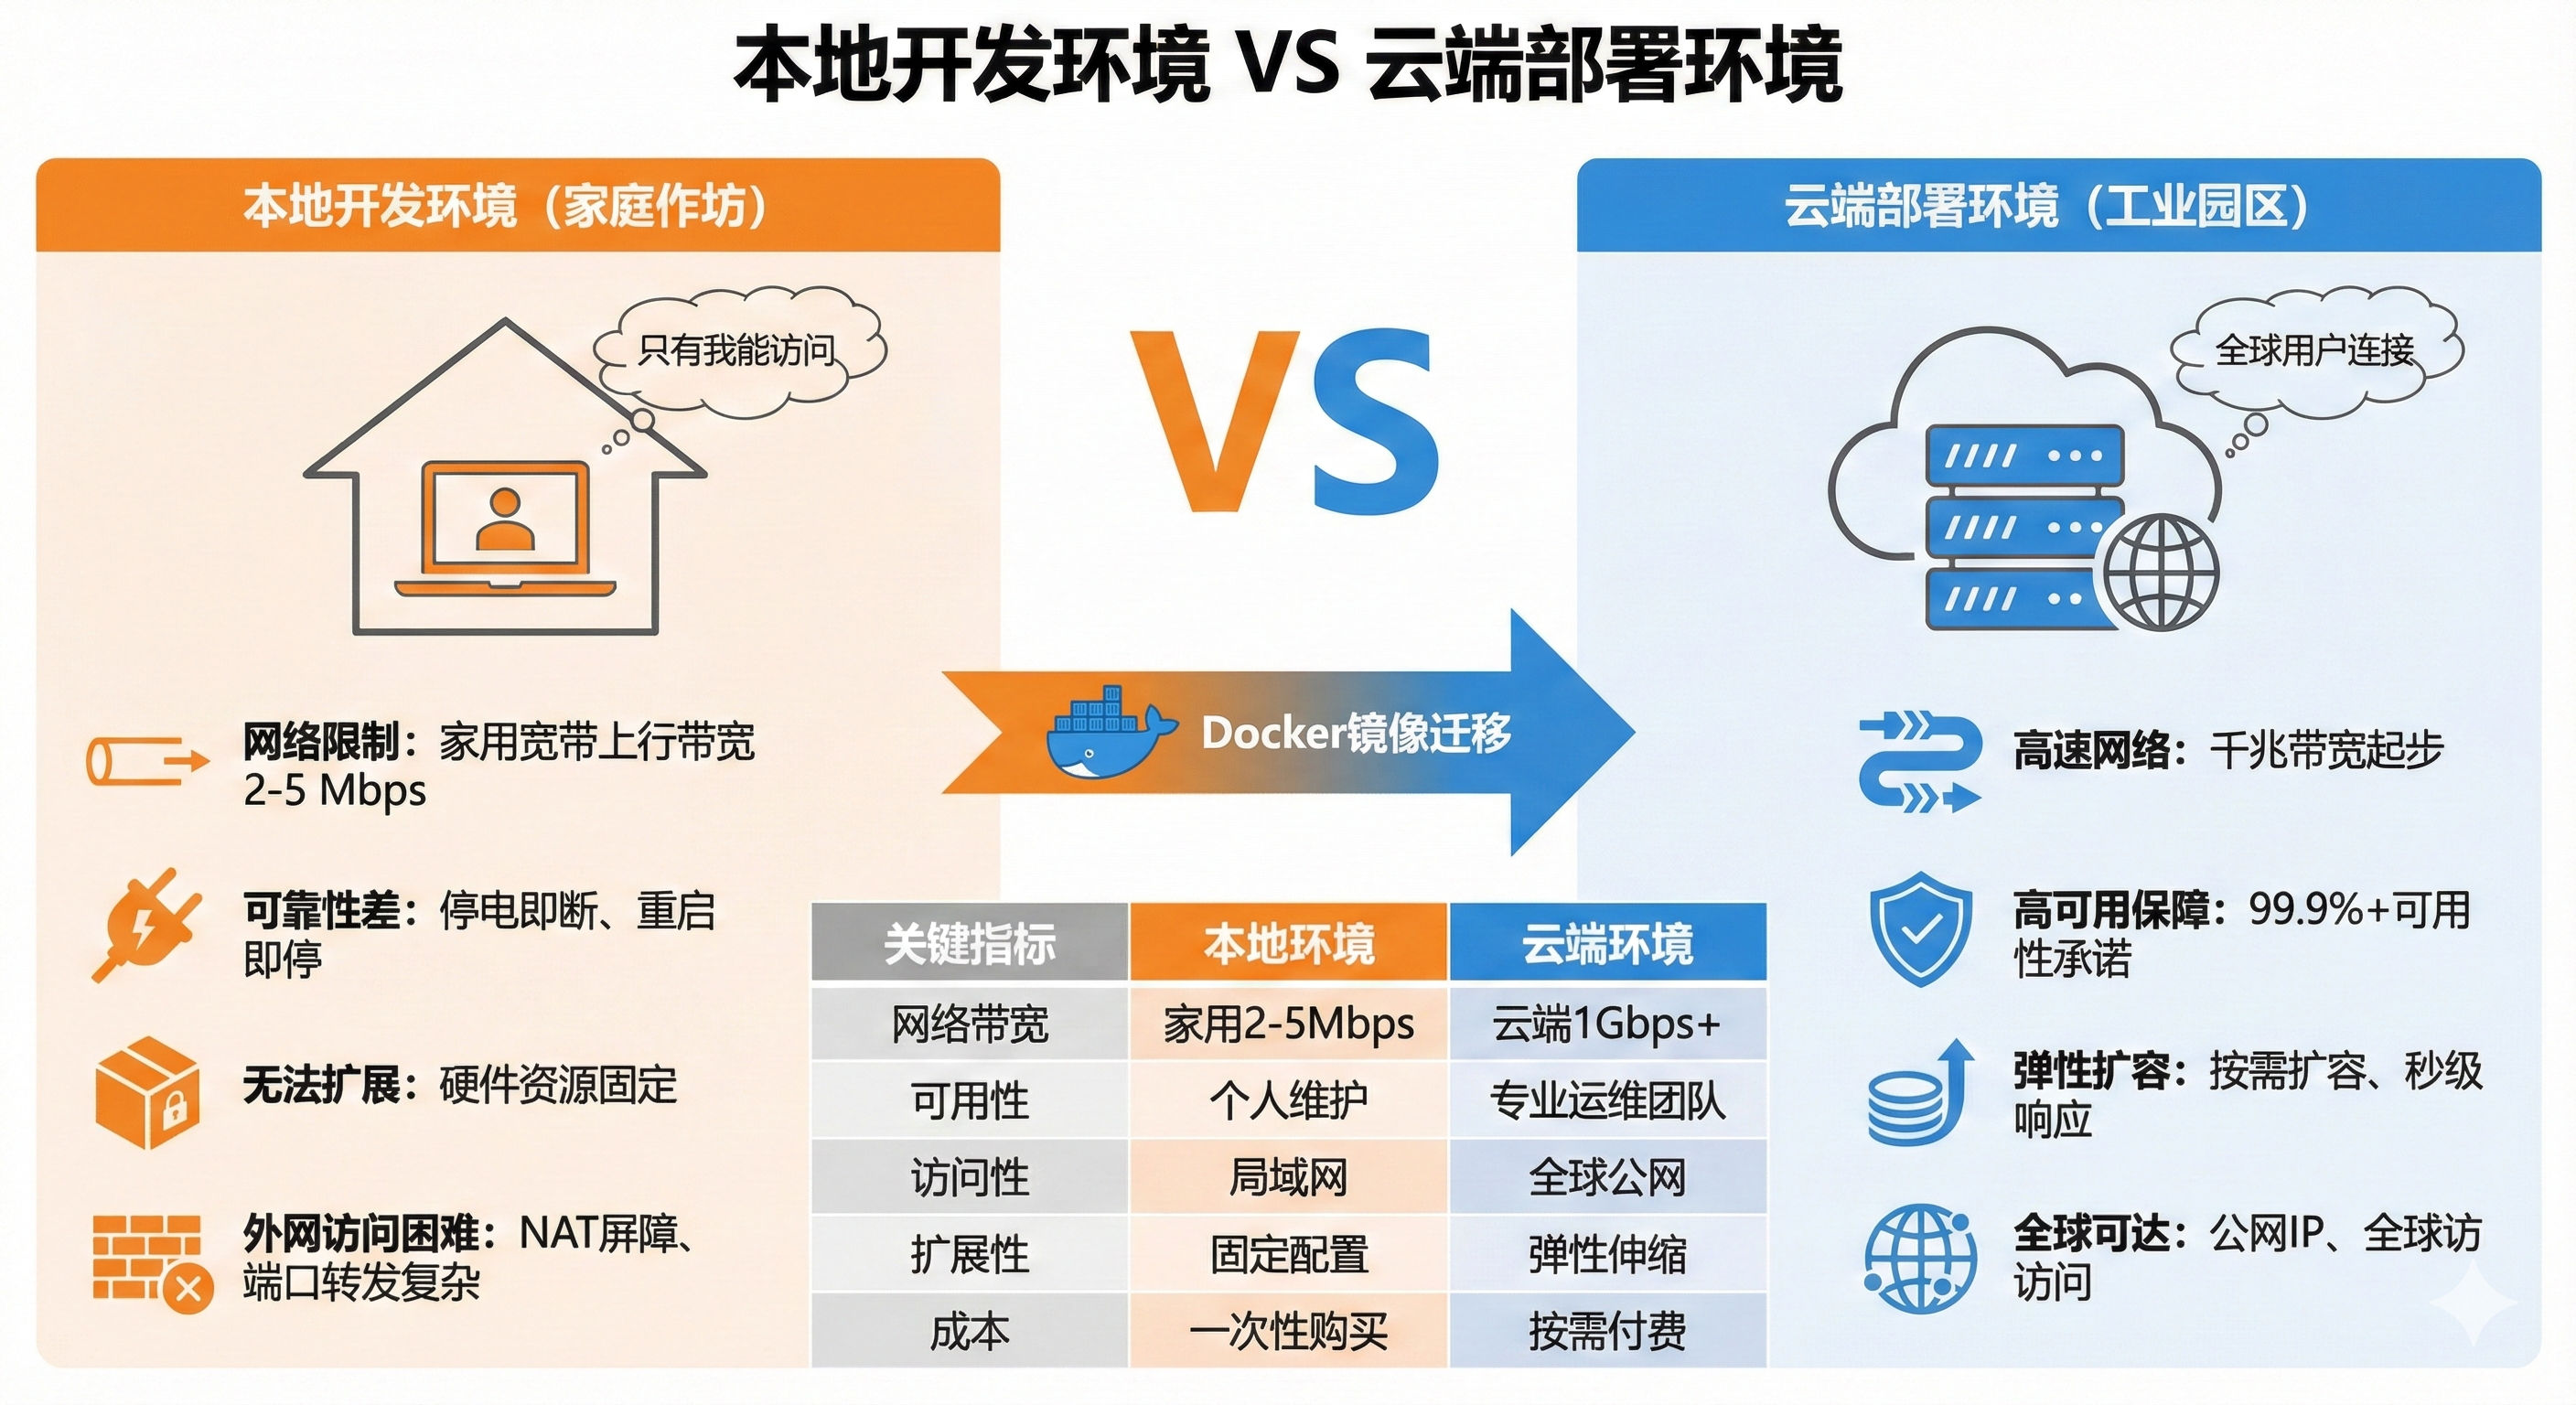
\includegraphics[width=0.9\textwidth]{figures/sec5/local-vs-cloud-environment.png}
\caption{本地开发环境与云端部署环境的全面对比}
\label{fig:local-vs-cloud}
\end{figure}

如图\ref{fig:local-vs-cloud}所示，从家庭作坊式的本地开发环境向工业级的云端部署环境迁移，不仅仅是硬件配置的提升，更是从个人实验向商业服务的根本转变。

\subsubsection{选择云端战场：配置你的虚拟战舰}

在决定将游戏世界搬到云端之后，我们面临的第一个实际问题就是：到底该选择什么样的云服务器？这个决策看似复杂，实际上可以用一个简单的对比来理解——就像从家里的小作坊升级到工业园区的标准厂房。

我们之前在本地开发时使用的个人电脑，就像是自己家里的一间小作坊：电源稳定性一般（停电就断），网络带宽有限（家用宽带上行只有几Mbps），而且只有你自己能进入（局域网访问）。更要命的是，一旦你的电脑关机或重启，整个“作坊”就停止运营了，所有的“客户”都会被拒之门外。

而云服务器则完全不同，它更像是工业园区里的标准化厂房：有不间断电源保障，配备高速光纤网络，24小时专业维护团队，全世界的客户都能轻松找到你的地址。最关键的是，如果业务扩张需要更大空间，你可以随时申请相邻的厂房进行扩容，而不用重新选址搬迁。

对于我们这种刚刚起步的游戏项目，配置选择其实并不复杂。大部分云厂商都提供了针对不同应用场景的推荐配置，我们只需要按照官方的入门指南来选择即可。通常来说，支持几十到几百名在线玩家的游戏服务，选择2-4核CPU、4-8GB内存的基础配置就足够了。操作系统建议选择Ubuntu 20.04 LTS，因为它对Docker的支持最为成熟，相关的教程和社区资源也最丰富。

更重要的是选择合适的地理位置。如果你的玩家主要在国内，选择华东或华北地区的数据中心能够提供最佳的网络延迟；如果面向海外玩家，则需要选择离目标用户更近的海外节点。这就像开实体店一样，位置的选择直接影响客流量和用户体验。

云服务器的真正价值不在于配置有多强大，而在于它提供的可靠性和可达性保障。当我们的游戏世界部署在云端后，它就变成了一个真正的“永不下线”的在线世界，全球的玩家都能随时随地进入并享受稳定的游戏体验。

\subsubsection{理解上云本质：从孤岛到互联网}

上云的核心不是简单的“换个地方放服务器”，而是一次架构思维的根本转变。在本地开发阶段，我们构建的是一个“孤岛式”的封闭系统：所有组件都在同一台机器上，通过本地网络通信，只有开发者能够访问。而上云意味着将这个封闭系统转变为开放的互联网服务，需要考虑的问题维度完全不同。

从技术架构角度看，上云过程实际上是在解决三个层次的连接问题。第一层是物理连接：确保云服务器具备稳定的网络接入能力，这包括带宽保障、延迟优化以及网络冗余等基础设施问题。第二层是逻辑连接：通过合理的端口映射和防火墙配置，让外部客户端能够正确找到并连接到我们的游戏服务。第三层是业务连接：确保服务在面对真实用户流量时能够稳定运行，这涉及并发处理、错误恢复、性能监控等运维层面的考虑。

更深层次地看，上云还意味着运维模式的转变。本地开发时，我们更多关注的是功能实现和逻辑正确性；而在云端环境中，服务的可观测性、可恢复性、可扩展性变得同样重要。这就需要我们在设计和部署服务时，从一开始就考虑日志收集、健康检查、优雅关闭等生产级特性。

\begin{figure}[htbp]
\centering
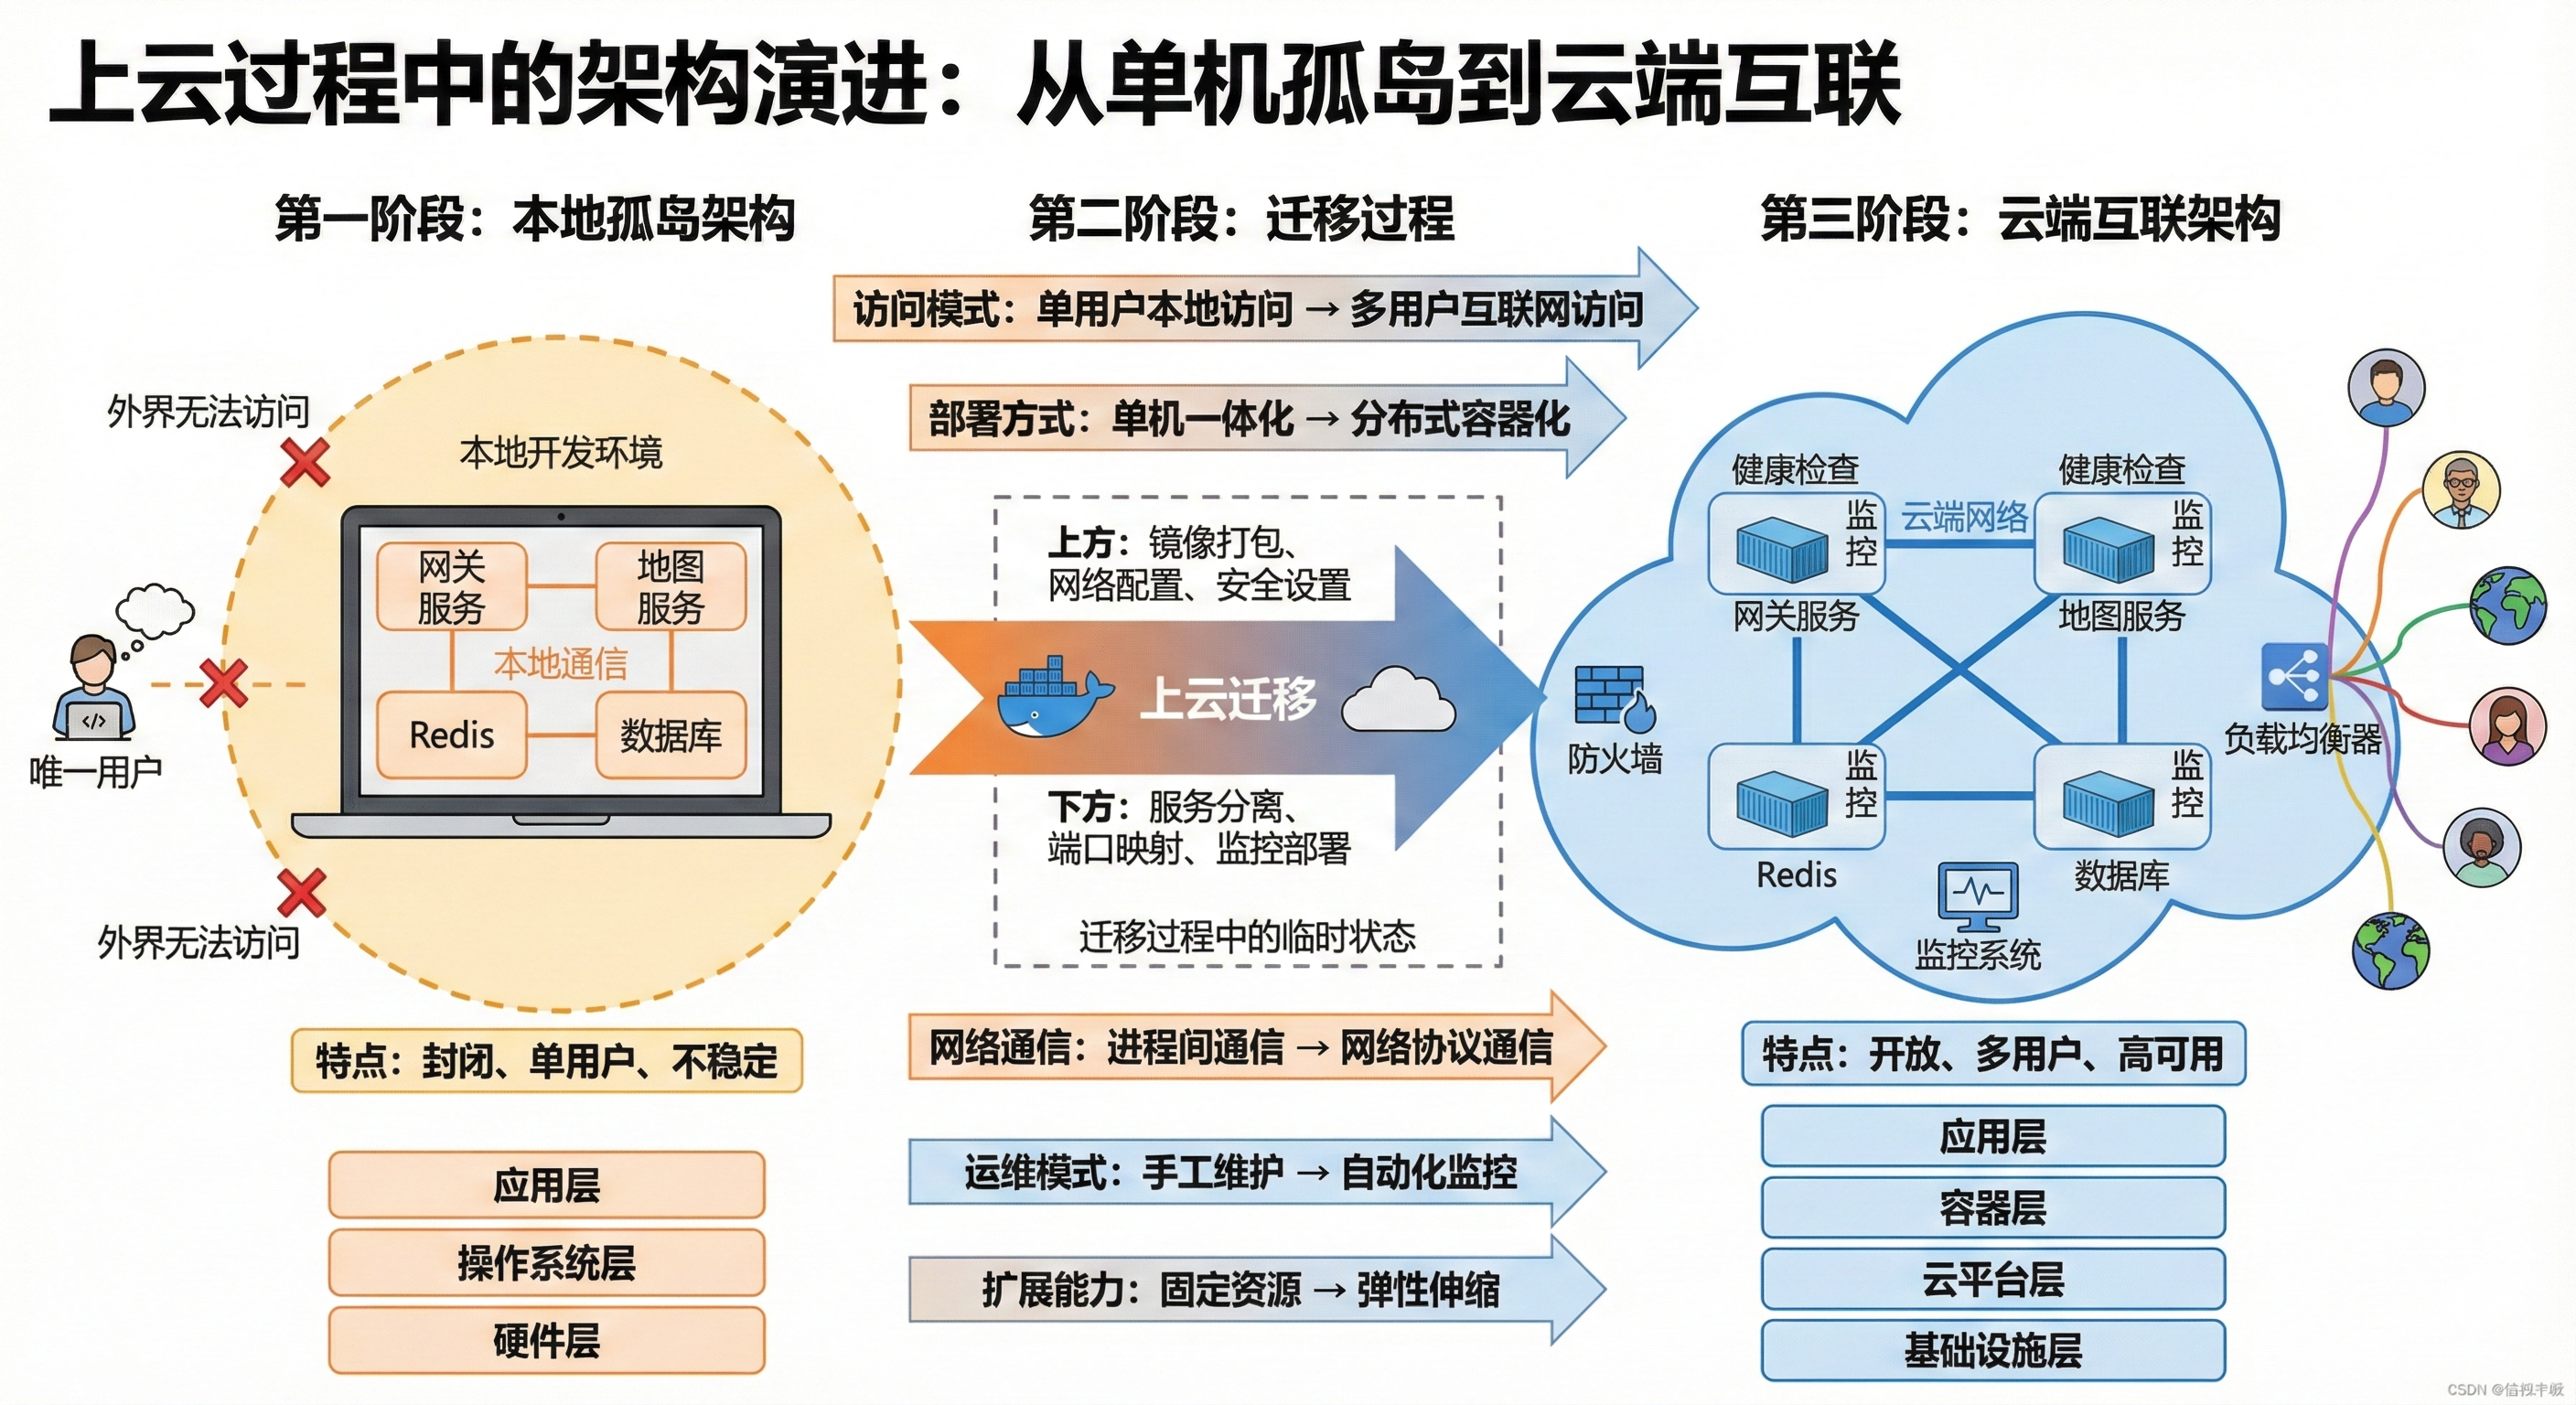
\includegraphics[width=0.9\textwidth]{figures/sec5/cloud-migration-architecture.png}
\caption{上云过程中的架构演进：从单机孤岛到云端互联}
\label{fig:cloud-migration}
\end{figure}

如图\ref{fig:cloud-migration}所示，上云不是简单的平移，而是整个系统架构从封闭走向开放、从静态走向动态的演进过程。

\subsubsection{镜像迁移：代码的跨环境旅行}

将我们在本地构建的Docker镜像传输到云端环境，是上云流程中最关键的技术环节。这个过程的本质是让我们的应用代码完成一次“跨环境旅行”，从开发者的本地机器迁移到云端的生产环境。

这个迁移过程面临着几个核心挑战。首先是传输效率问题：Docker镜像通常体积较大，从几百MB到几个GB不等，如何在有限的网络带宽下快速可靠地完成传输，直接影响部署效率。其次是版本一致性问题：如何确保云端运行的镜像与本地构建的镜像完全一致，避免因为环境差异导致的运行时问题。最后是安全性问题：在镜像传输和存储过程中，如何保护应用代码和敏感配置不被泄露。

最推荐的做法是利用镜像仓库机制来实现镜像的分发。这个过程类似于我们使用应用商店下载手机APP：开发者先将应用上传到商店（推送镜像到仓库），用户再从商店下载到自己设备（从仓库拉取镜像到云服务器）。

镜像仓库的核心优势在于其分层存储机制。Docker镜像本质上是由多个层（Layer）叠加而成的，当我们推送镜像时，仓库会智能地识别哪些层是新的、哪些层是重复的。这意味着后续的版本更新只需要传输变化的部分，大大提升了传输效率。

在选择镜像仓库时，我们有多种选择。Docker Hub是最常用的公共仓库，免费用户可以创建无限数量的公开镜像，但私有镜像数量有限制。各大云厂商也提供了自己的容器镜像服务，如阿里云的容器镜像服务ACR、腾讯云的容器镜像服务TCR等，这些服务通常提供更好的国内访问速度和更丰富的企业级功能。

\begin{figure}[htbp]
\centering
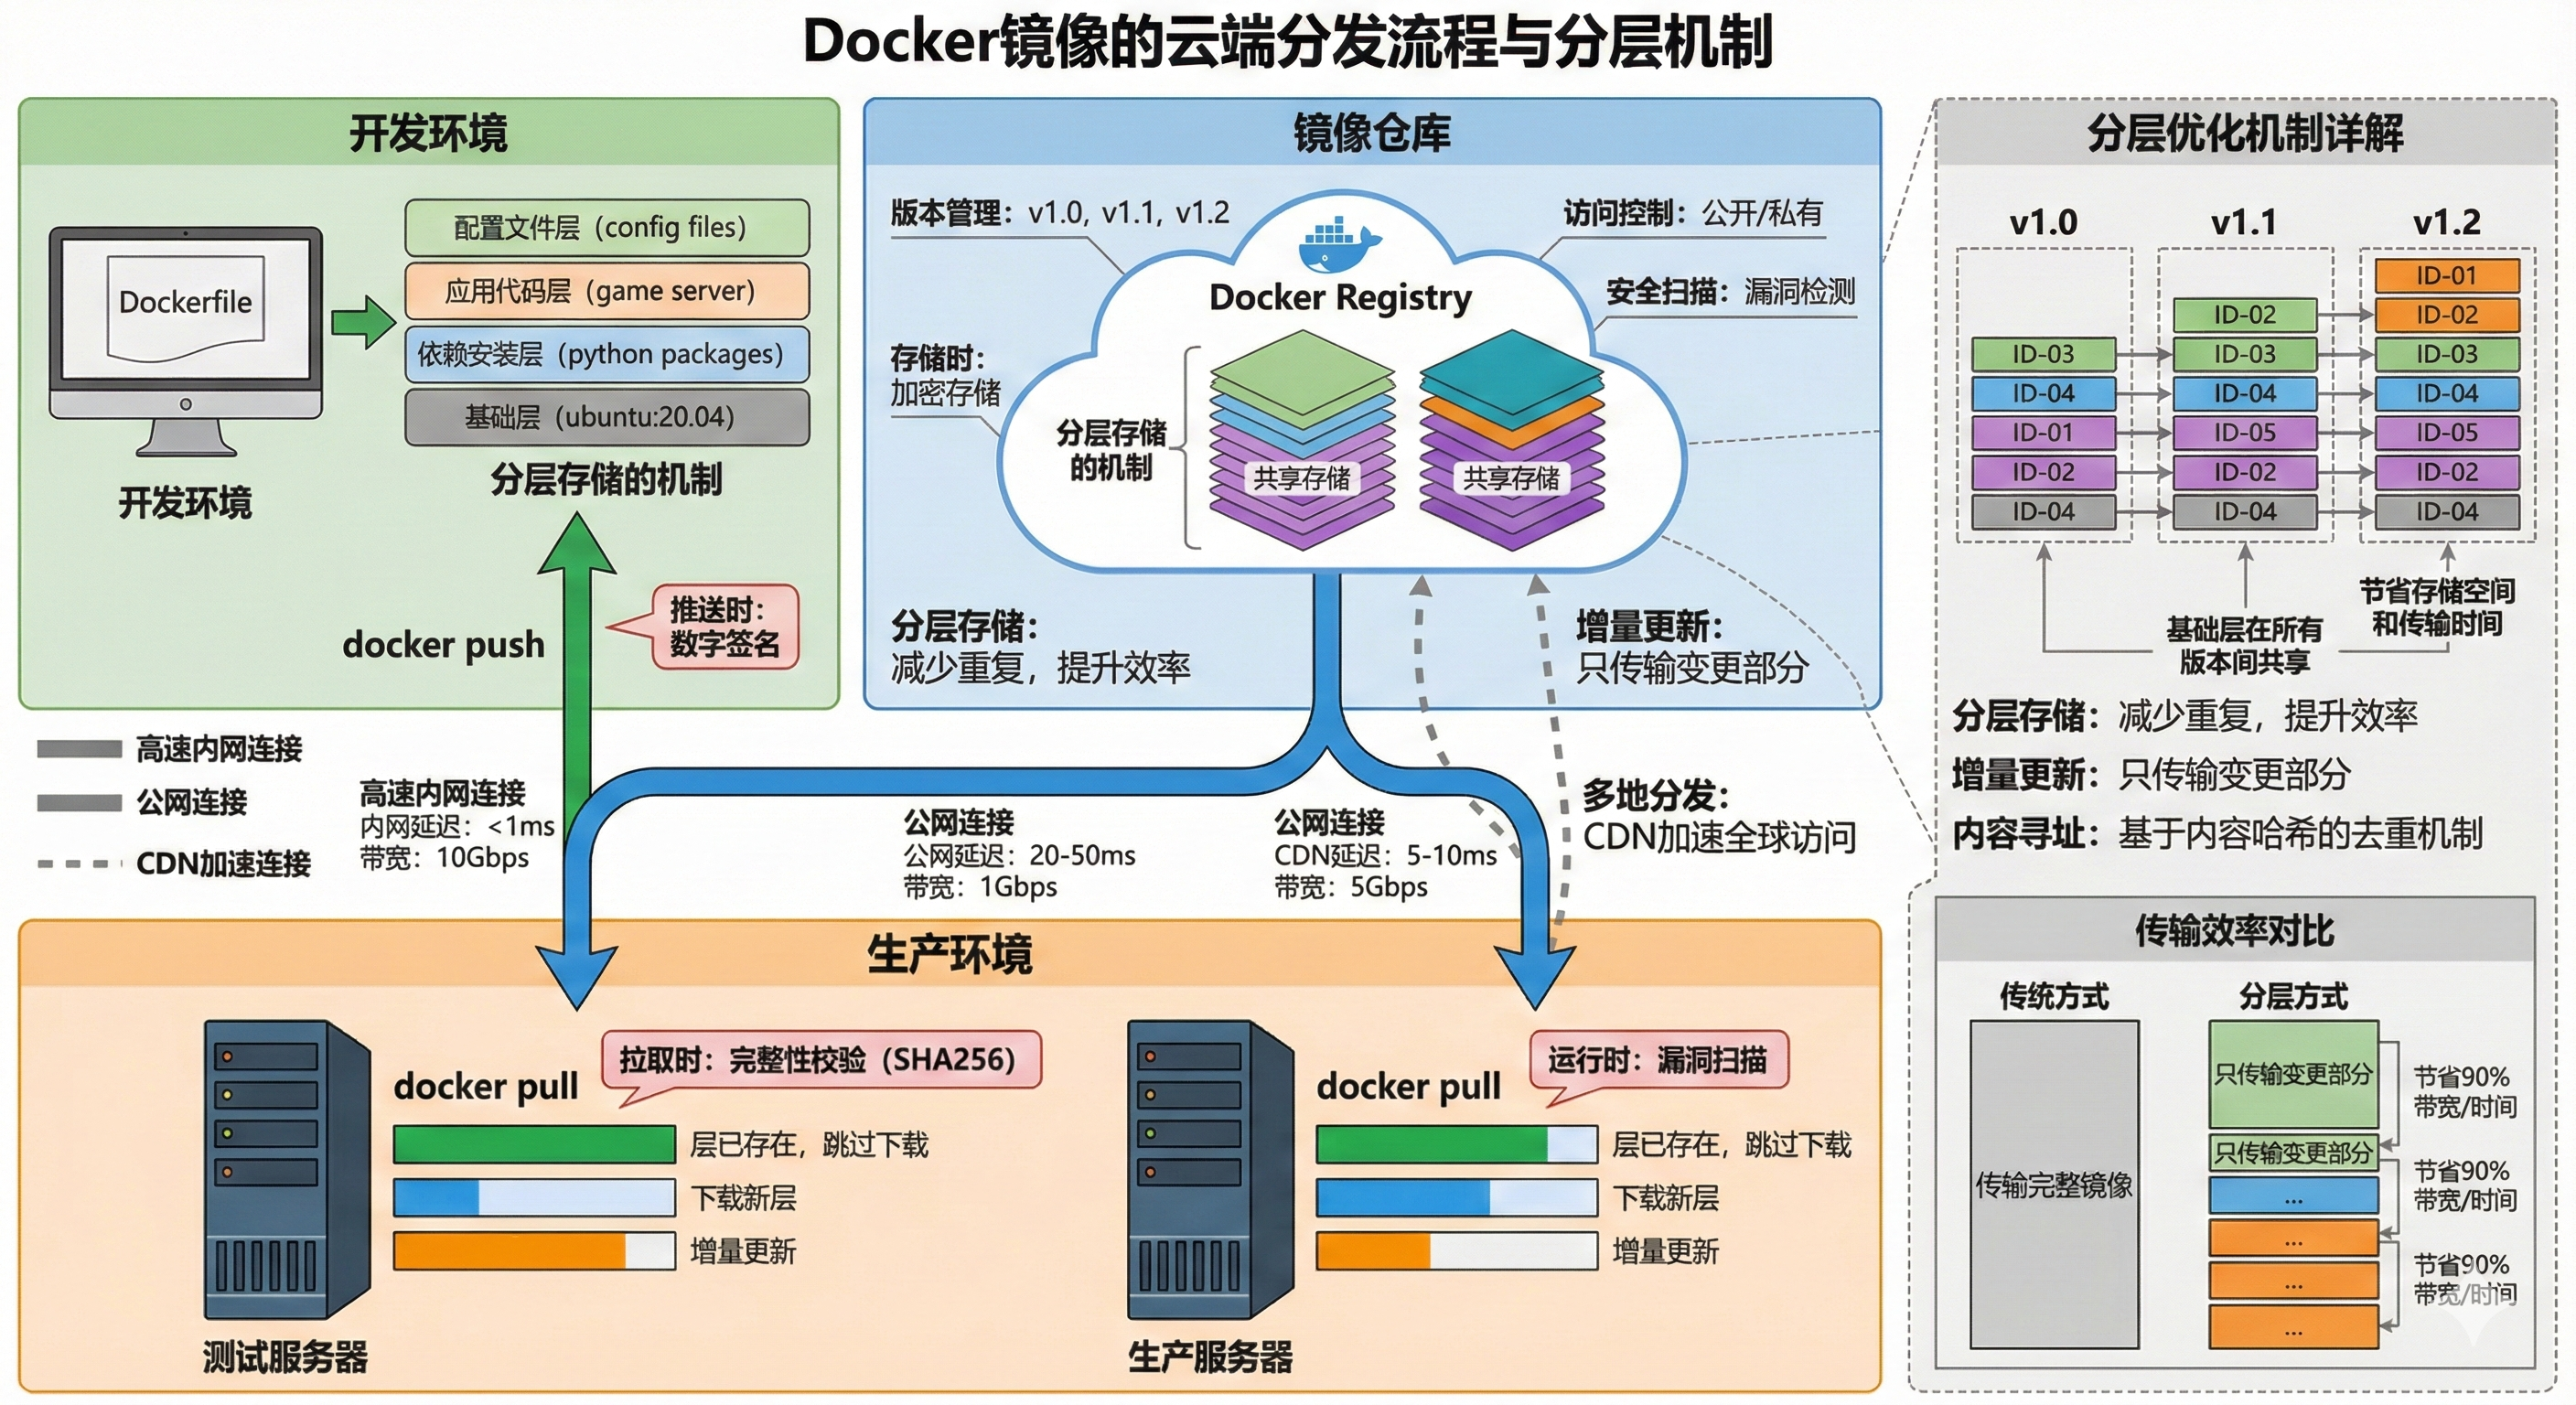
\includegraphics[width=0.9\textwidth]{figures/sec5/docker-image-distribution.png}
\caption{Docker镜像的云端分发流程与分层机制}
\label{fig:image-distribution}
\end{figure}

对于对安全性要求较高或网络环境特殊的场景，也可以选择直接文件传输的方式。这种方法将镜像导出为文件，然后通过文件传输工具将其上传到云服务器，最后重新导入镜像。虽然这种方式缺乏仓库机制的便利性，但在某些企业内网环境或对数据流向有严格管控的场景下，这种点对点传输方式反而更加合适。

无论采用哪种传输方式，都强烈建议在传输完成后进行完整性校验。通过比较本地和远程镜像的摘要值，可以确保传输过程中没有发生数据损坏。这种看似多余的验证步骤，往往能在关键时刻避免因为镜像损坏导致的莫名其妙的运行时错误。

\subsubsection{网络配置：为服务打开通往世界的大门}

成功将镜像传输到云端并启动服务后，最后一个关键步骤就是配置网络访问策略。如果说镜像迁移是让应用“安家落户”，那么网络配置就是为这个新家“开门接客”的过程。

云环境的网络安全机制相比本地环境要严格得多，遵循的是“默认拒绝，显式允许”的安全原则。这意味着新启动的云服务器几乎所有端口都是关闭的，我们需要根据业务需求，显式地为每个需要对外提供服务的端口开放访问权限。

云厂商通常通过“安全组”（Security Group）机制来管理网络访问规则。安全组本质上是一套网络防火墙规则的集合，可以精确控制哪些来源IP、哪些端口、哪些协议被允许访问你的服务器。

安全组的工作原理类似于小区的门禁系统。你需要为每类访客（不同类型的网络请求）制定不同的准入规则：普通访客（游戏玩家）可以通过大门（游戏端口）进入；快递员（监控系统）可以通过特定入口（监控端口）送货；而维修人员（运维管理）则需要特殊权限（SSH端口）才能进入核心区域。

对于我们的游戏服务，通常需要配置以下几类规则：HTTP/HTTPS端口用于网页版游戏或API接口访问，WebSocket端口用于实时通信，以及可能的自定义端口用于游戏专有协议。这些服务端口通常需要向全球开放，以便世界各地的玩家都能访问。同时，SSH管理端口应该严格限制访问来源，只允许运维人员的固定IP地址访问。如果架构中包含多台服务器之间的内部通信，这些端口只需要对内网其他服务器开放。

\begin{figure}[htbp]
\centering
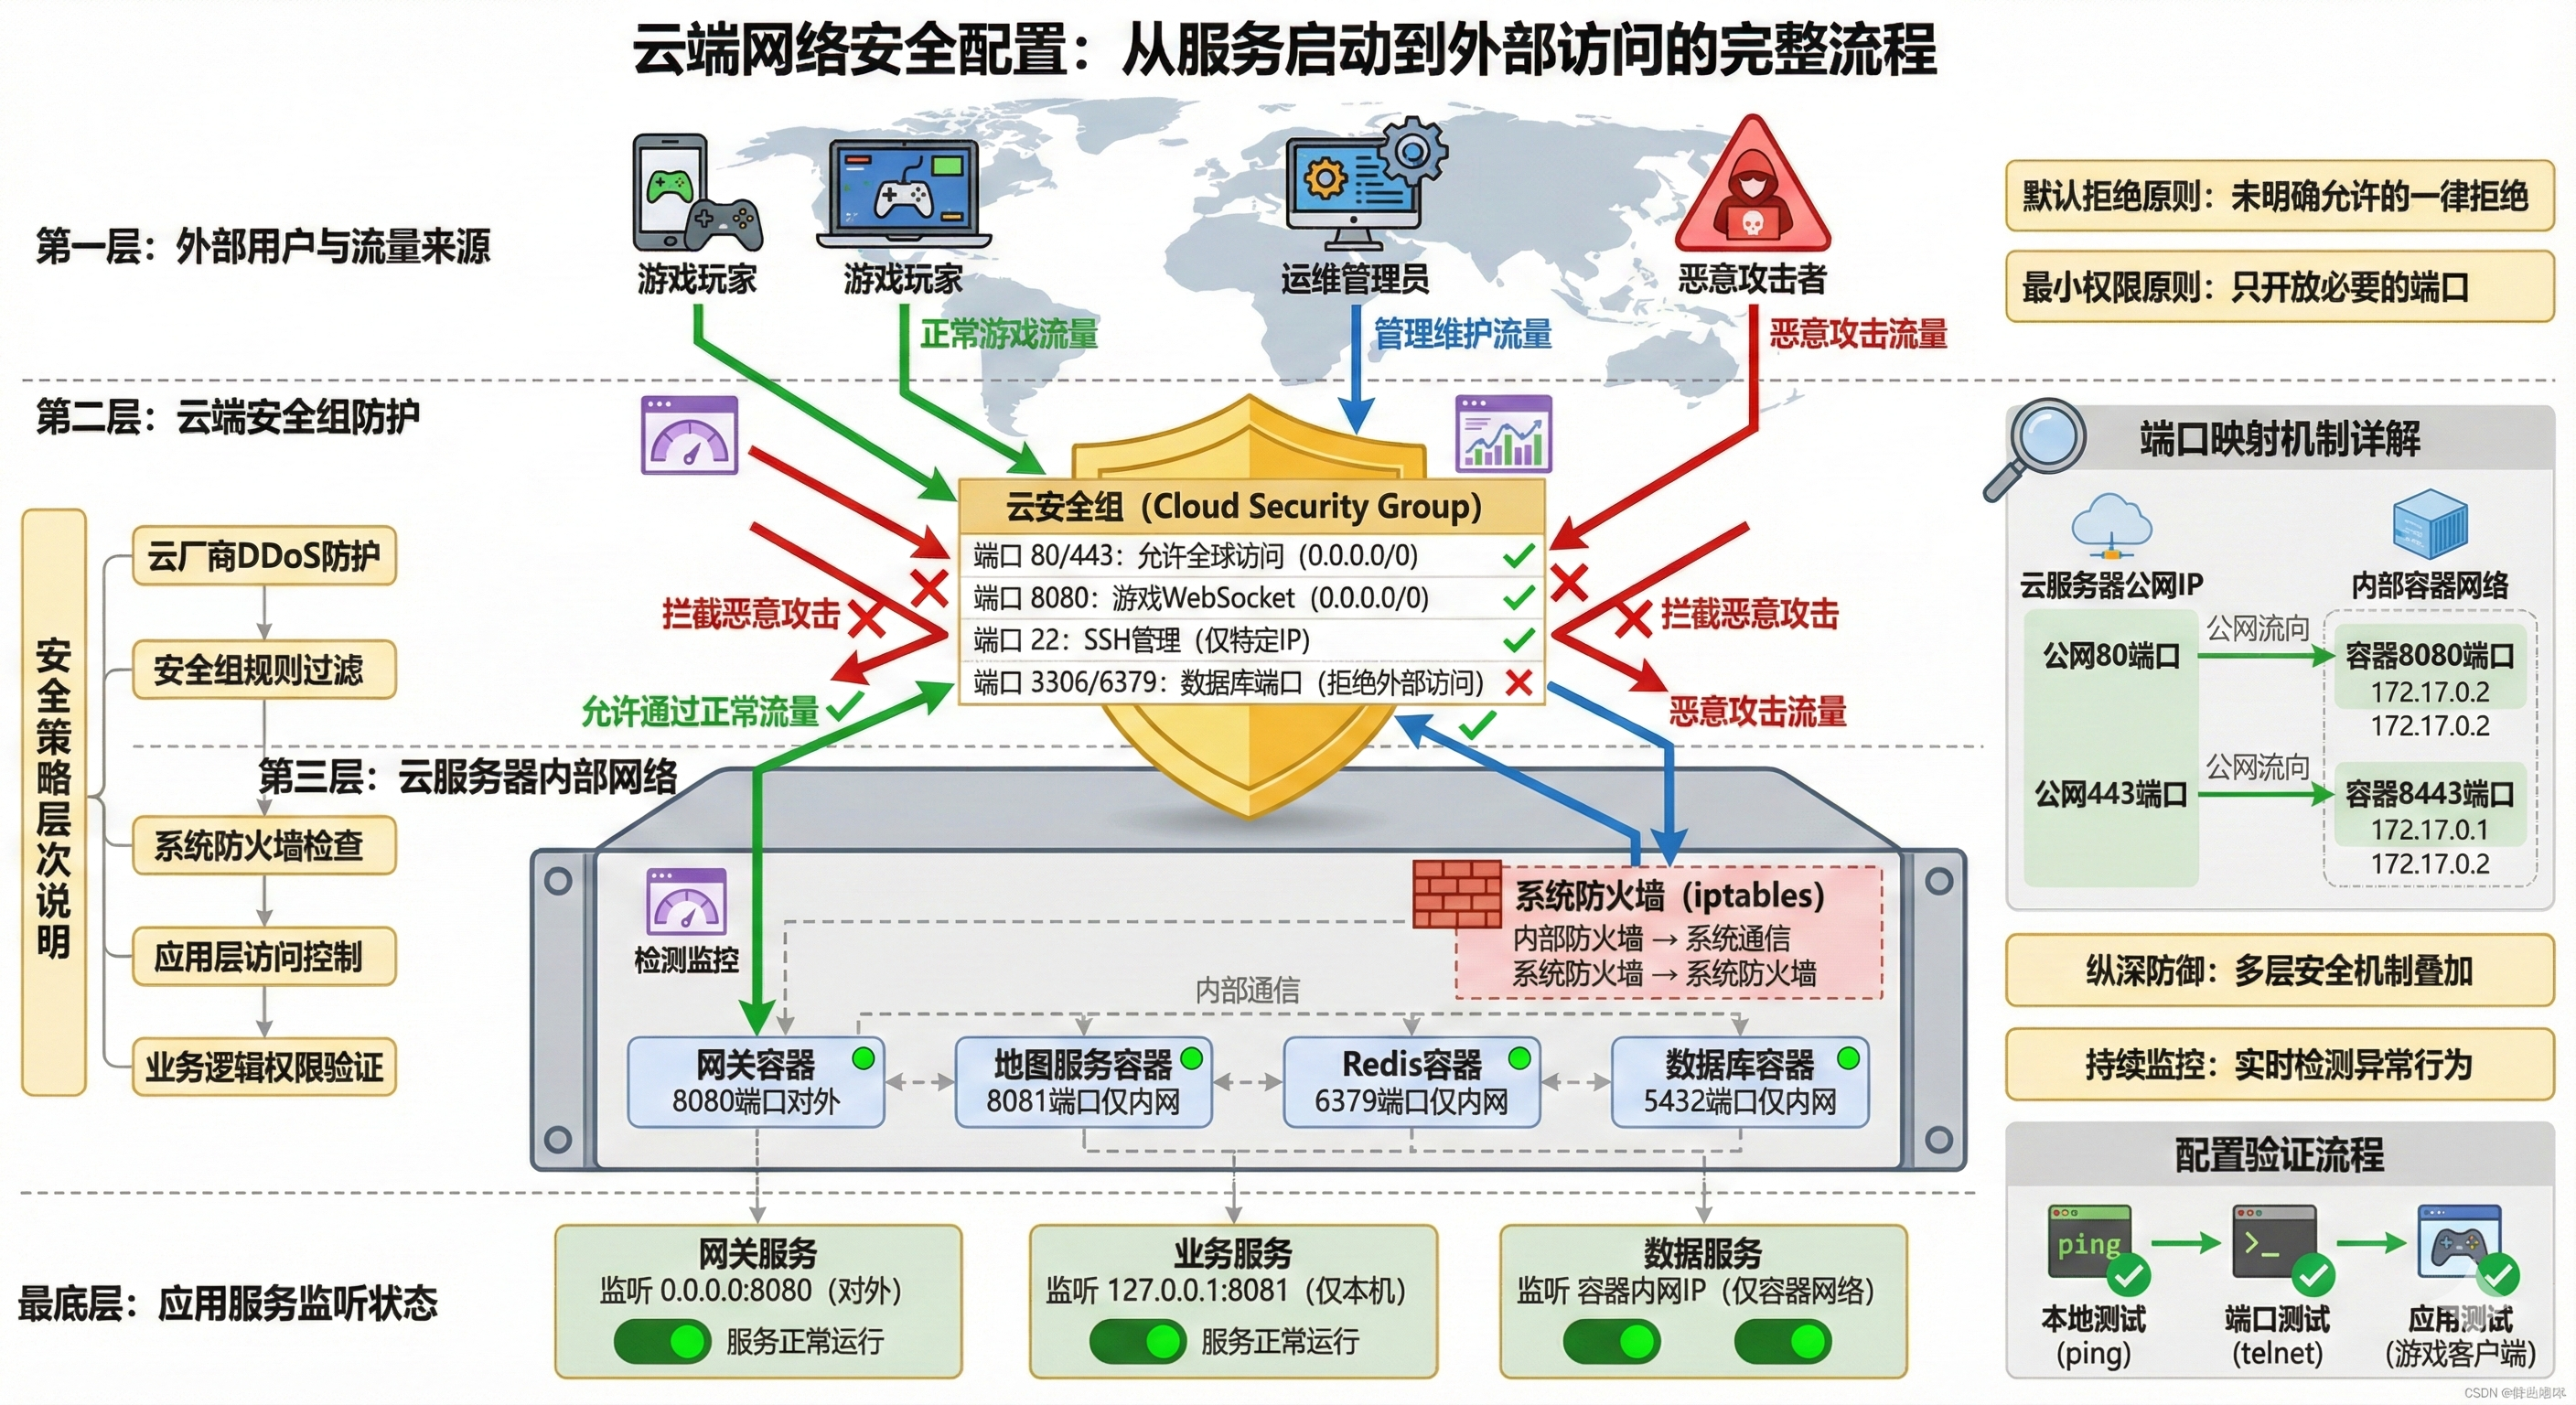
\includegraphics[width=0.9\textwidth]{figures/sec5/cloud-network-security.png}
\caption{云端网络安全配置：从服务启动到外部访问的完整流程}
\label{fig:network-security}
\end{figure}

配置完安全组规则后，强烈建议进行端到端的连通性测试。这个过程就像检查水管是否通畅一样，我们需要确保数据包能够顺利地从外部客户端传输到我们的游戏服务。

测试方法可以从简单到复杂逐步进行。最基础的测试是检查服务器是否可达；进一步可以测试特定端口是否开放；最完整的测试是从实际的游戏客户端发起连接，验证整个应用层协议是否正常工作。

在测试过程中，如果发现连接问题，需要逐层排查：首先检查云服务器的安全组配置是否正确；然后检查服务器内部的防火墙设置；最后确认游戏服务本身是否正常运行并监听在正确的端口上。

通过云端监控工具观察服务器的网络流量、连接数、响应时间等关键指标，也能帮助我们及时发现和解决网络问题。当看到监控面板上出现来自全球各地的连接请求时，就意味着我们的游戏世界真正向全世界开放了。

\subsubsection{从概念到现实：完成上云的最后一跃}

通过以上四个步骤——认识上云价值、选择云端资源、迁移应用镜像、配置网络访问——我们成功地将游戏服务从本地环境迁移到了云端。这不仅仅是一次简单的环境迁移，更是从个人项目向互联网服务的根本转变。

这种转变带来的影响是深远的。从技术角度看，我们获得了更强的可靠性、更好的性能表现、以及面向未来的扩展能力；从产品角度看，游戏从一个只有开发者能体验的原型，变成了全球玩家都能访问的实际服务；从团队角度看，这为后续的协作开发、持续集成、运维监控等工程化实践奠定了基础。

然而，上云只是万里长征的第一步。真正的工业级应用还需要考虑高可用架构、自动化运维、弹性伸缩、灾难恢复等更复杂的技术问题。在接下来的章节中，我们将进一步探索如何利用容器编排、微服务治理等先进技术，让我们的游戏服务具备真正的企业级运维能力。

当你的游戏服务在云端稳定运行，来自世界各地的玩家开始涌入你精心构建的虚拟世界时，那种从创意到现实的成就感，正是每一个技术创造者最珍贵的回报。云端部署不仅仅是技术的升级，更是梦想照进现实的关键一步。

\subsection{Dockerfile逐行详解}
\label{sec:appendix-dockerfile}

本节对第五章5.1节中展示的通用Dockerfile进行逐行解读，帮助读者理解每条指令的具体作用。

这份Dockerfile采用"分层多阶段构建"技术，将整个流程划分为"编译"与"运行"两个阶段。

第1--9行是编译阶段，目标是利用完整的工具链将源代码转化为可执行的二进制文件。第1行与第2行引入包含Go编译器等所有开发工具的官方镜像，命名为builder便于后续引用。3--4行是关键优化：利用Docker基于文件内容的缓存机制，配合Go的依赖管理文件（go.mod）与校验文件（go.sum），只要依赖没有变化，Docker就会直接跳过下载步骤，实现"秒级"热启动。源代码放在依赖构建之后复制，是因为源代码改动最频繁，而Docker的缓存机制是逐层叠加的——如果把源代码放在依赖之前，缓存就会失效。6--7行定义了针对传入参数的服务构建分流逻辑，同时避免构建出空壳镜像。第9行进行静态编译，生成的可执行文件自带所有依赖库，不依赖操作系统的动态链接库，这也是容器可以部署在极简环境中的原因。

后续是生产环境阶段。第10行选择Alpine作为底座，这是一个只有5MB左右的极简镜像。第11行安装时区数据，修正容器默认的UTC时间，确保服务器能正确处理北京时间。14--15行是构建过程的精髓：\texttt{COPY --from=builder}仅从第一阶段提取编译好的可执行文件与配置文件，将源代码和编译器全部丢弃。最后一行定义容器启动时默认执行的命令。

\subsection{Kubernetes部署实战}
\label{sec:appendix-k8s-deploy}

本节将第五章5.4节中的实战操作步骤独立出来，供读者在理解K8s核心概念后动手实践。

理解了Kubernetes的工作原理后，让我们通过实际的部署过程来体验其强大能力。整个部署过程体现了"声明期望，自动实现"的云原生理念。

部署准备的第一步是确保镜像资源就绪。我们需要将游戏服务的Docker镜像推送到Kubernetes集群可以访问的镜像仓库中。这个步骤延续了我们在容器化阶段建立的标准化流程，确保集群中的任何Node都能获取到相同的镜像版本。

第二步是编写声明式配置文件。Kubernetes使用YAML格式的配置文件来描述期望状态，这些配置文件包含了资源定义、依赖关系、约束条件等所有必要信息。对于我们的游戏服务，主要需要定义Deployment和Service两类资源。

\begin{figure}[htbp]
\centering
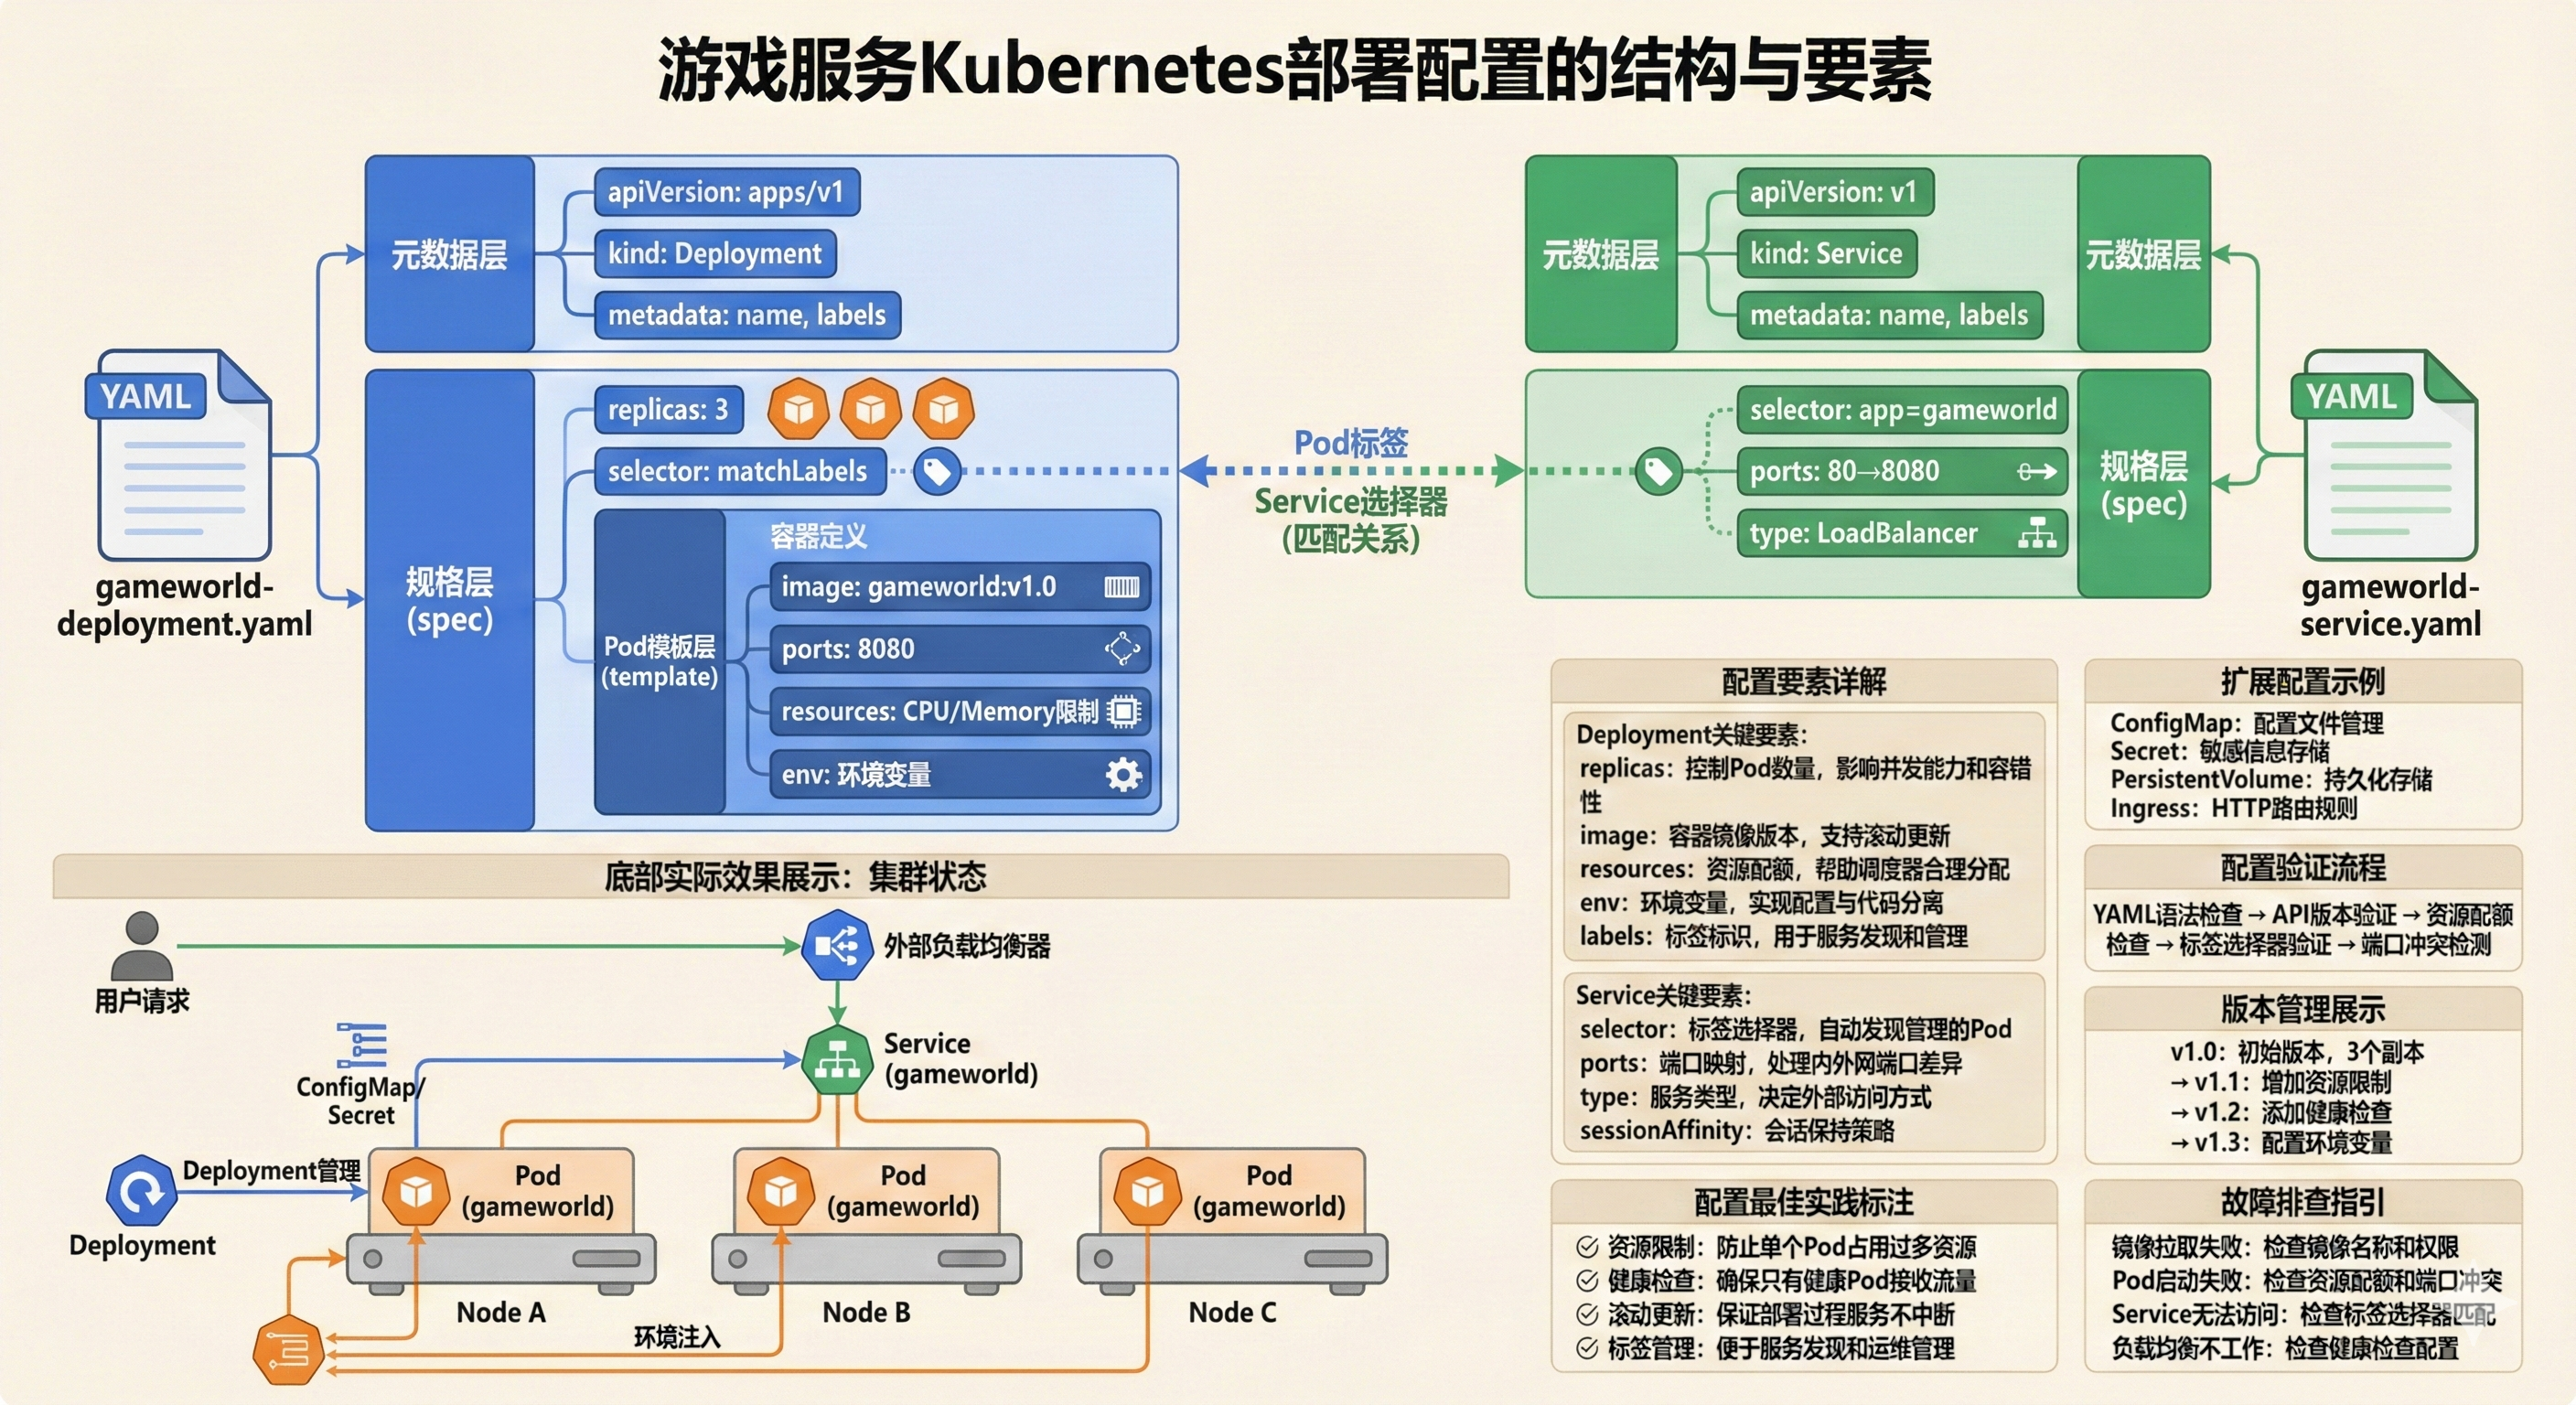
\includegraphics[width=0.9\textwidth]{figures/sec5/kubernetes-deployment-configuration.png}
\caption{游戏服务Kubernetes部署配置的结构与要素}
\label{fig:k8s-config}
\end{figure}

如图\ref{fig:k8s-config}所示，Deployment配置定义了Pod模板、副本数量、更新策略、资源限制等关键参数。副本数量决定了系统的并发处理能力和容错级别；资源限制帮助调度器进行合理的资源分配；更新策略确保版本升级时的服务连续性。这种配置方式将复杂的运维决策转化为了清晰的参数设置，大大降低了出错的可能性。

Service配置定义了服务的网络暴露方式、端口映射、负载均衡策略等。通过标签选择器机制，Service能够自动发现并管理所有相关的Pod，形成统一的访问入口。负载均衡器的自动配置让外部流量能够均匀分配到所有健康的Pod实例上，实现了高可用和高性能。

第三步是执行部署命令。通过kubectl命令行工具，我们可以将配置文件提交给Kubernetes API服务器。一旦配置被接受，整个集群就会开始协调工作来实现期望状态。我们可以通过各种kubectl命令来监控部署进度、查看资源状态、调试问题。

\begin{figure}[htbp]
\centering
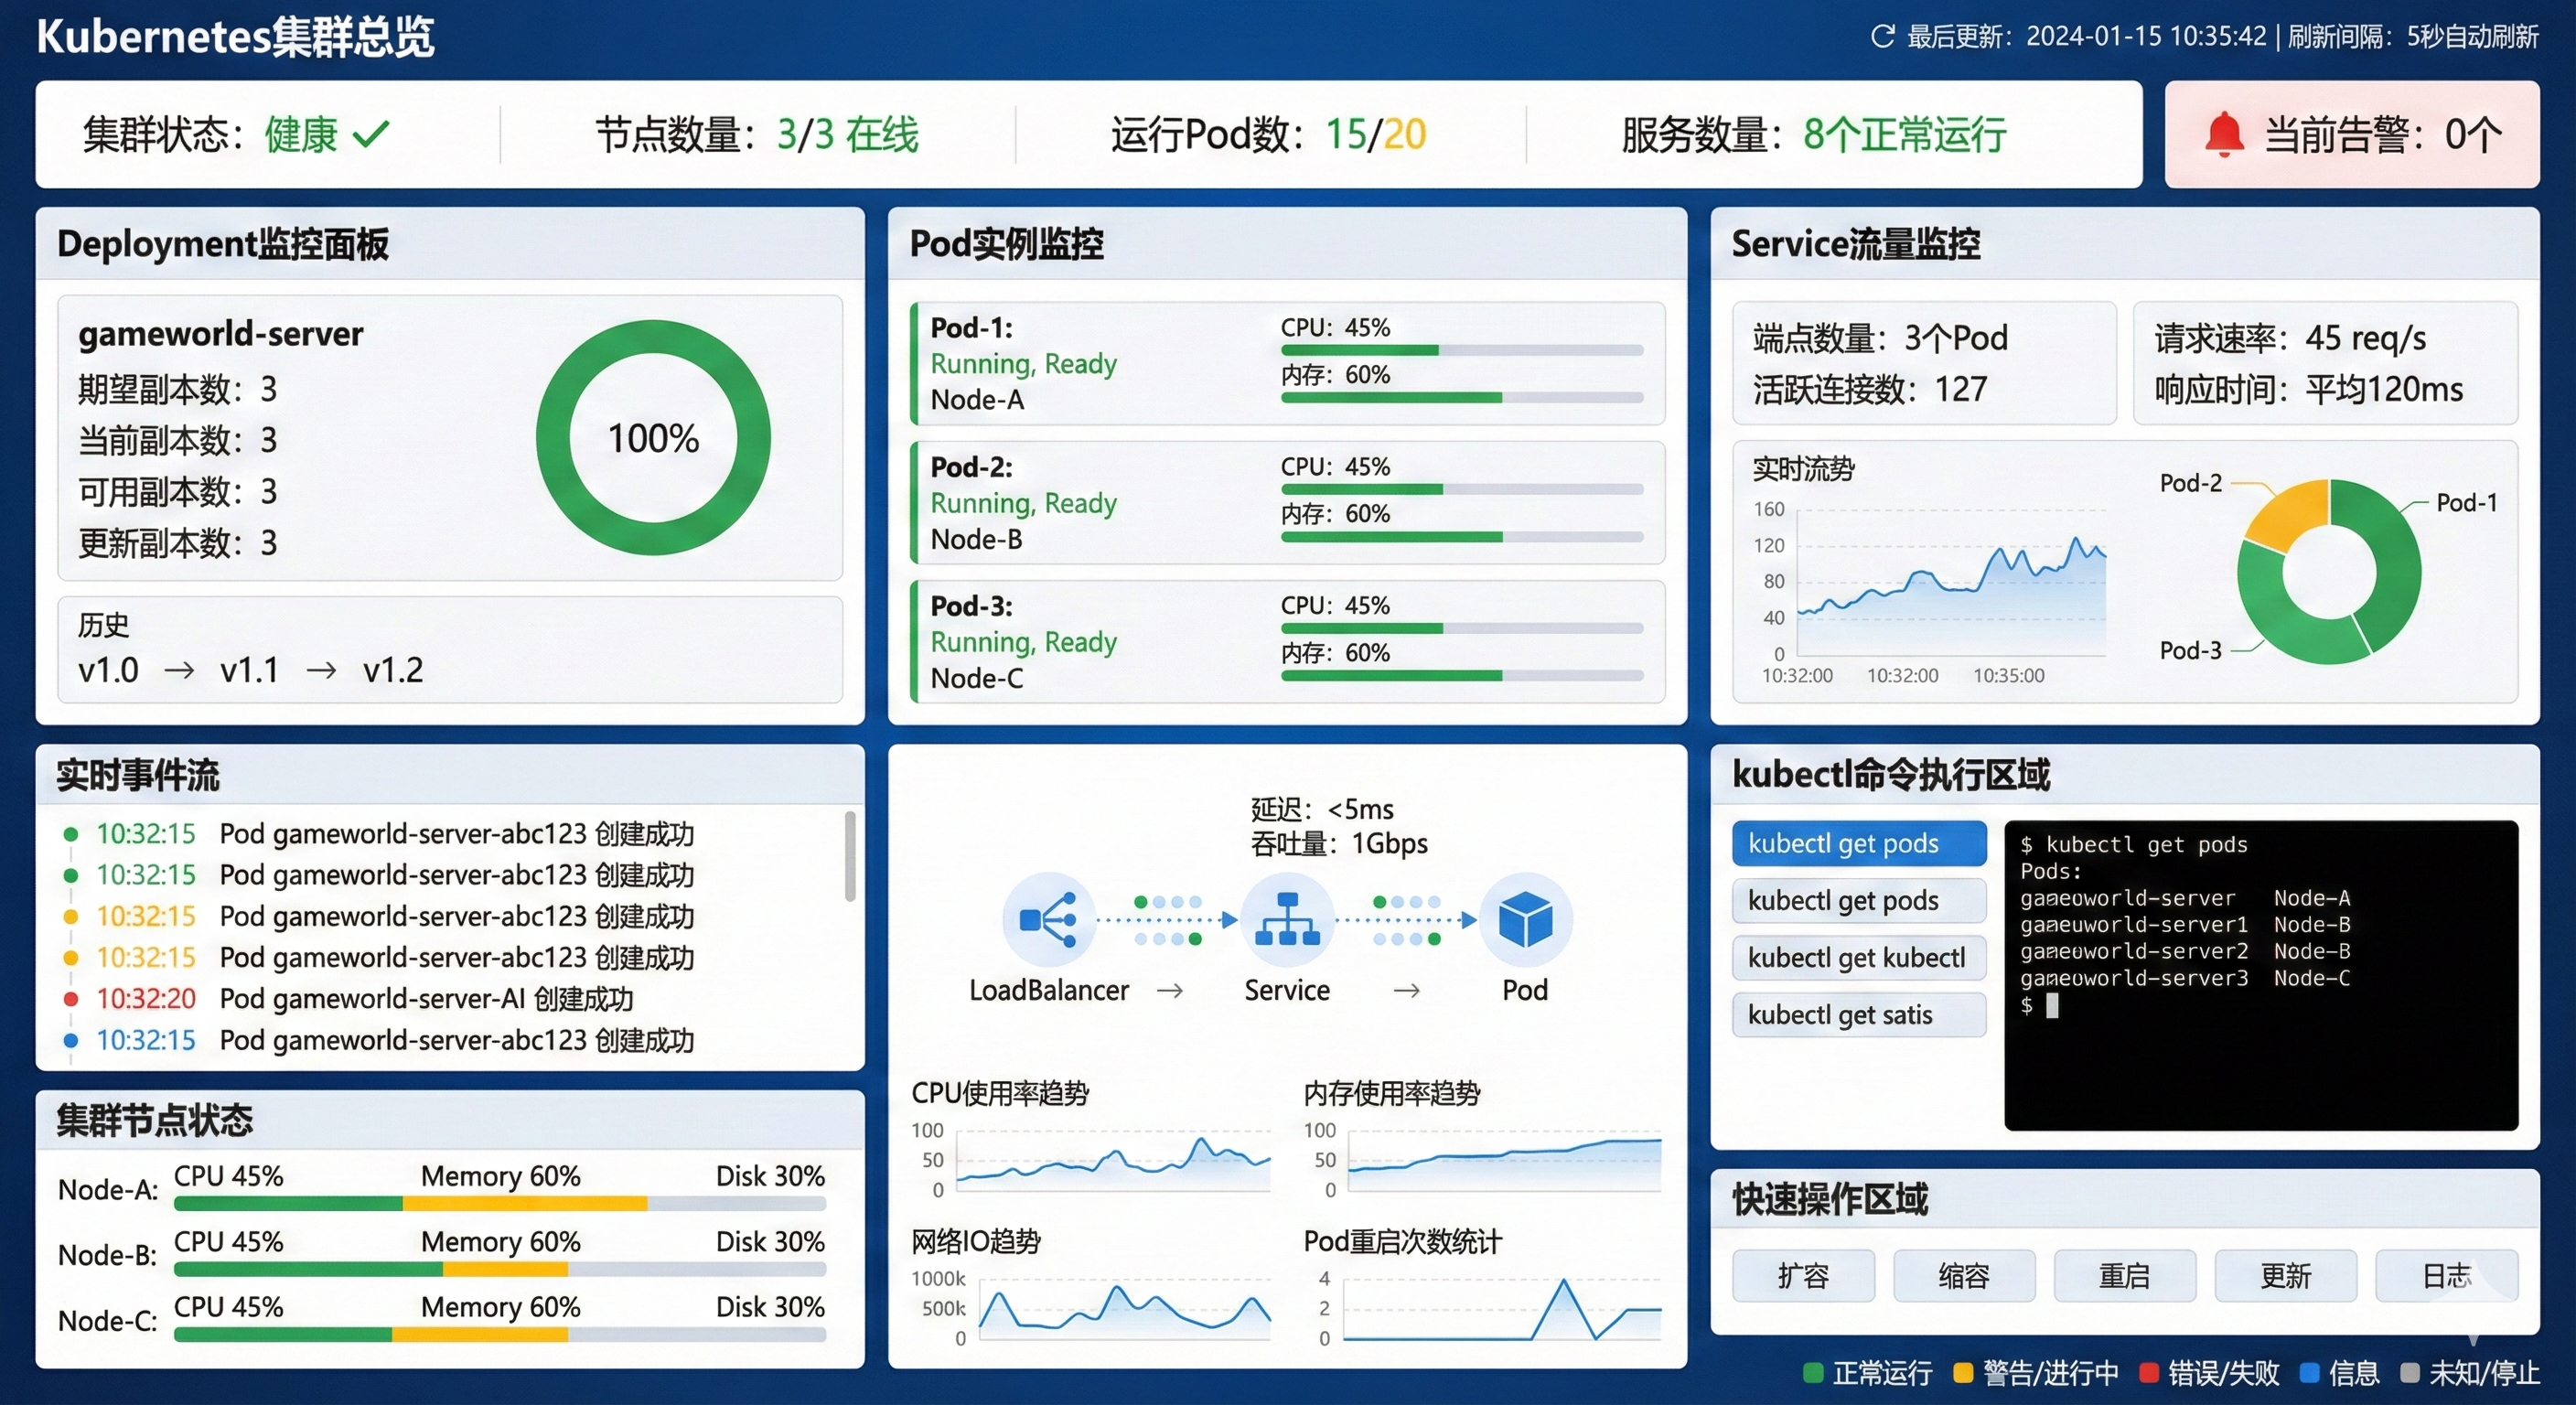
\includegraphics[width=0.9\textwidth]{figures/sec5/kubernetes-deployment-monitoring.png}
\caption{Kubernetes部署过程的监控与状态查看}
\label{fig:k8s-monitoring}
\end{figure}

如图\ref{fig:k8s-monitoring}所示，部署完成后，我们就获得了一个高度自动化的服务运行环境。当需要扩容时，只需修改配置文件中的副本数并重新应用；当需要更新服务版本时，只需修改镜像标签并执行滚动更新；当某个Pod出现故障时，Kubernetes会自动重启或替换。这种自动化程度让运维工作从"被动响应"转变为"主动配置"，大大提升了效率和可靠性。

通过这一节的学习，我们已经掌握了Kubernetes的核心理念和基本使用方法。但这仅仅是容器编排世界的入门，Kubernetes还提供了配置管理、服务网格、监控告警等更高级的功能。

当你看到kubectl命令返回"deployment successfully deployed"的提示时，意味着你已经成功将应用从单机模式升级到了分布式集群模式。此时的游戏服务不再依赖于单台服务器的稳定性，而是由整个Kubernetes集群的智能调度和自动恢复能力来保障，这是向云原生架构迈出的关键一步。
